%%% LaTeX Template: Article/Thesis/etc. with colored headings and special fonts
%%%
%%% Source: http://www.howtotex.com/
%%% Feel free to distribute this template, but please keep to referal to http://www.howtotex.com/ here.
%%% February 2011
%%%
%%% Modified January 2016 by CDM

%%%  Preamble
\documentclass[11pt,letterpaper]{article}
\usepackage[margin=1.0in]{geometry}
\usepackage[T1]{fontenc}
\usepackage[bitstream-charter]{mathdesign}
\usepackage[latin1]{inputenc}					
\usepackage{amsmath}						
\usepackage{xcolor}
\usepackage{cite}
\usepackage{hyphenat}
\usepackage{graphicx}
\usepackage{float}
\usepackage{subfigure}
\usepackage{sectsty}
\usepackage[compact]{titlesec} 
\usepackage[tablegrid]{vhistory}
\usepackage{pbox}
\allsectionsfont{\color{accentcolor}\scshape\selectfont}

%%% Definitions
%%%%%%%%%%%%%%%%%%%%%%%%%%%%%%%%%%%%%%%%%%%%%%%%%%%%
% UPDATE THIS SECTION TO YOUR TEAM AND SEMESTER INFO
\definecolor{accentcolor}{rgb}{0.0,0.0,0.5} 
\newcommand{\teamname}{Runtime Terror}
\newcommand{\productname}{Turing Board}
\newcommand{\coursename}{CSE 4317: Senior Design II}
\newcommand{\semester}{Spring 2022}
\newcommand{\docname}{Detailed Design Specification}
\newcommand{\department}{Department of Computer Science \& Engineering}
\newcommand{\university}{The University of Texas at Arlington}
\newcommand{\authors}{Sahaj Amatya \\ Sarker Nadir Afridi Azmi \\ Kendall Buchanan \\ Keaton Koehler \\ Happy Ndikumnaa \\ Lydia Sarver}

%%% Headers and footers
\usepackage{fancyhdr}
	\pagestyle{fancy}						% Enabling the custom headers/footers
\usepackage{lastpage}	
	% Header (empty)
	\lhead{}
	\chead{}
	\rhead{}
	% Footer
	\lfoot{\footnotesize \teamname \ - \semester}
	\cfoot{}
	\rfoot{\footnotesize page \thepage\ of \pageref{LastPage}}	% "Page 1 of 2"
	\renewcommand{\headrulewidth}{0.0pt}
	\renewcommand{\footrulewidth}{0.4pt}

%%% Change the abstract environment
\usepackage[runin]{abstract}			% runin option for a run-in title
%\setlength\absleftindent{30pt}			% left margin
%\setlength\absrightindent{30pt}		% right margin
\abslabeldelim{\quad}	
\setlength{\abstitleskip}{-10pt}
\renewcommand{\abstractname}{}
\renewcommand{\abstracttextfont}{\color{accentcolor} \small \slshape}	% slanted text

%%% Start of the document
\begin{document}

%%% Cover sheet
%%%%%%%%%%%%%%%%%%%%%%%%%%%%%%%%%%%%%%%%%%%%%%%%%%%%%%%%%%%%%%%%%%%%%%%%%%%%
%   CHANGE THE GRAPHIC HERE. PUT YOUR IMAGE IN THE 'images' 
%   FOLDER AND UPDATE THE NAME FROM 'images/test_image' TO YOUR IMAGE NAME
{\centering \huge \color{accentcolor} \sc \textbf{\department \\ \university} \par}
\vspace{0.5 in}
{\centering \huge \color{accentcolor} \sc \textbf{\docname \\ \coursename \\ \semester} \par}
\vspace{0.3 in}
\begin{figure}[h!]
	\centering
   	
\includegraphics[width=0.60\textwidth]{images/turing_logo} 
\end{figure}
\vspace{0.2 in}
{\centering \huge \color{accentcolor} \sc \textbf{\teamname \\ \productname} \par}
\vspace{0.3 in}
{\centering \large \sc \textbf{\authors} \par}
\newpage


%\vspace{1 in}
%\centerline{January 13th, 2012}
%\newpage

%%% Revision History
%%%%%%%%%%%%%%%%%%%%%%%%%%%%%%%%%%%%%%%%%%%%%%%%%%%%%%%%%%%%%%%%%
%   EACH '\vhEntry' BEGINS A ROW; EACH {} IS A COLUMN. UPDATE
%   THIS TO REFLECT YOUR REVISION HISTORY
\begin{versionhistory}
  	\vhEntry{0.1}{3.09.2022}{KB|LS|SA|HN|KK|SA}{First Draft}
  	\vhEntry{0.2}{3.11.2022}{KB|LS}{First Edit}
\end{versionhistory}
\newpage

%%% Table of contents
\setcounter{tocdepth}{2}
\tableofcontents
\newpage

%%% List of figures and tables (optional)
\listoffigures
\listoftables
\newpage

%%% Document sections
%%%%%%%%%%%%%%%%%%%%%%%%%%%%%%%%%%%%%%%%%%%%%%%%%%%%%%%%%%%%%%%
%   THIS IMPORTS LATEX FILES FROM THE TEX FOLDER. COPY/PASTE TO
%   ADD SECTIONS AS NEEDED AND CREATE FILE FOR IT IN TEX FOLDER
\section{Introduction}
Your introduction should provide a brief overview of the product concept and a reference to the requirement specification and architectural design documents in 1 or 2 paragraphs. The purpose is to provide the reader with the location of relevant background material that lead to the design details presented in this document.

\section{System Overview}
The main controls layer is in charge of processing and sending out the majority of the signals on the Turing Board. It uses the Jetson TX2 to communicate with the microprocessor in the wheels and turning layer to control the wheels and turning mechanism. There are several sensors in the wheels and turning layer that send information via the microprocessor to the Jetson as inputs. The Jetson also receives inputs from the power layer to know how much power is left in the battery. The last input to the Jetson comes from the Human Machine Interface (HMI) layer. This layer consists of items used to allow the Turing Board to understand the world around it and operate more appropriately. Along with the human machine interface layer, the computer vision layer also contributes to the Jetson TX2 receiving feedback from its environment. The computer vision layer uses RGB imagery and stereo and infrared imagery to see obstacles and the user depending on the mode it is currently in. Finally, the remote control for the Turing Board allows the user to control the board as an electric longboard when in the respective mode. The app boasts many features including user authentication and ride data analysis.

%%%%%%%%%%%%%%%%%%%%%%%%%%%%%%%%%%%%%%%%%%%%%%%%%%%%%%%%%%%%%%%%%%%%%%%%%%%%%%%%%%%%%%%%%%%%%
% If you want to change the image, put your image in the images folder and change "data_flow" 
% to the name of your image. You can also change the caption (System architecture) to 
% something else if you want.
\begin{figure}[h!]
	\centering
 	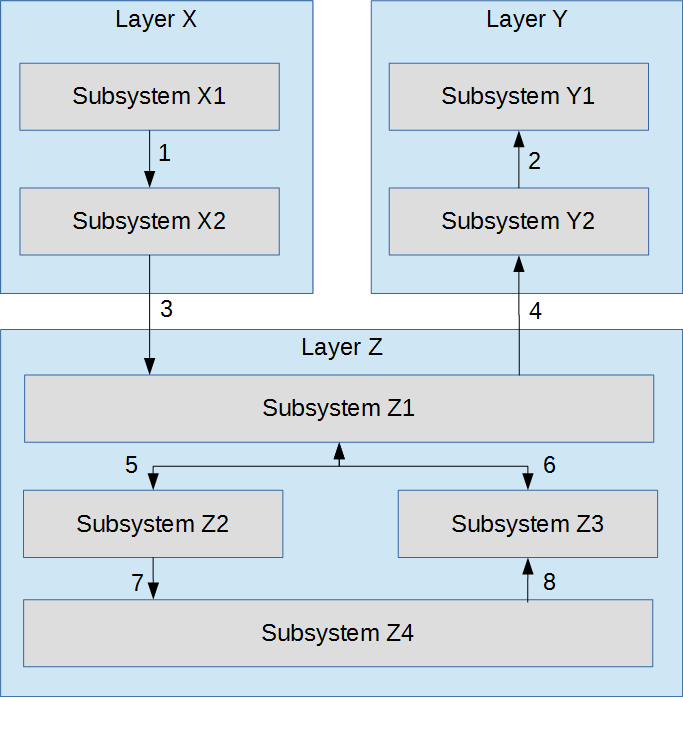
\includegraphics[width=0.90\textwidth]{images/data_flow} % Change me
 \caption{System Architecture}
\end{figure}

\newpage
%\section{Subsystem Definitions \& Data Flow}
%This section breaks down your layer abstraction to another level of detail. Here you grapically represent the logical subsytems that compose each layer and show the interactions/interfaces between those subsystems. A subsystem can be thought of as a programming unit that implements one of the major functions of the layer. It, therefore, has data elements that serve as source/sinks for other subsystems. The logical data elements that flow between subsystems need to be explicitly defined at this point, beginning with a data flow-like diagram based on the block diagram.

%%%%%%%%%%%%%%%%%%%%%%%%%%%%%%%%%%%%%%%%%%%%%%%%%%%%%%%%%%
%  BE SURE TO UPDATE THE IMAGE CAPTION
\begin{figure}[h!]
	\centering
 	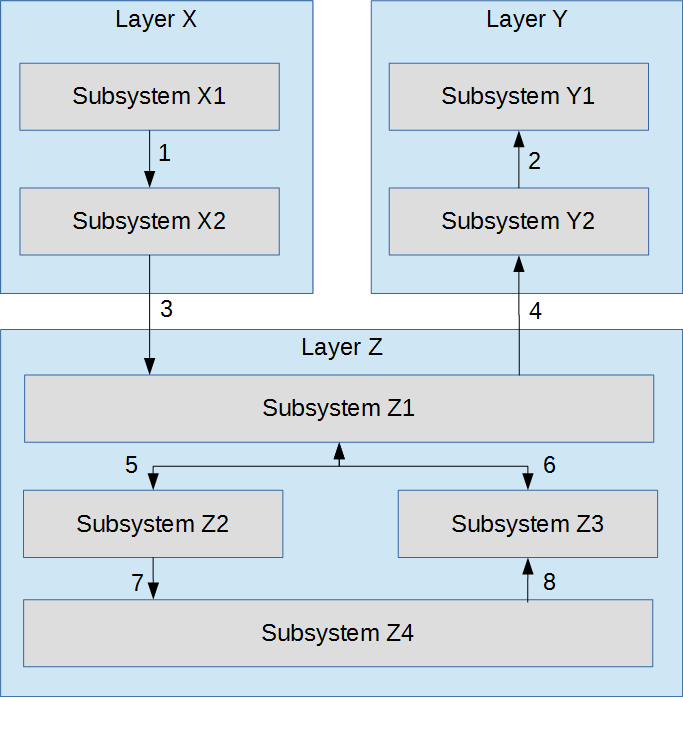
\includegraphics[width=\textwidth]{images/data_flow} % Image
 \caption{A simple data flow diagram} % Caption
\end{figure}

\newpage
\section{Power Layer Subsystems}
Each electrical component has a specific power requirement and this layer is responsible for providing that power.

\subsection{Layer Hardware}
The Turing Board includes an ER 36 volt battery and Songhe LM2596S Buck Converters. 

\subsection{Layer Operating System}
No operating system is used in this layer.

\subsection{Layer Software Dependencies}
No software is used in this layer.

\subsection{Subsystem 1}
This module consists of a Li-Po battery which provides power to a Buck Converter. It is an ER 36 volt battery with a 30A current output.

%%%%%%%%%%%%%%%%%%%%%%%%%%%%%%%%%%%%%%%%%%%%%%%%%%%%%%%%%%
%  BE SURE TO UPDATE THE IMAGE CAPTION
\begin{figure}[h!]
	\centering
 	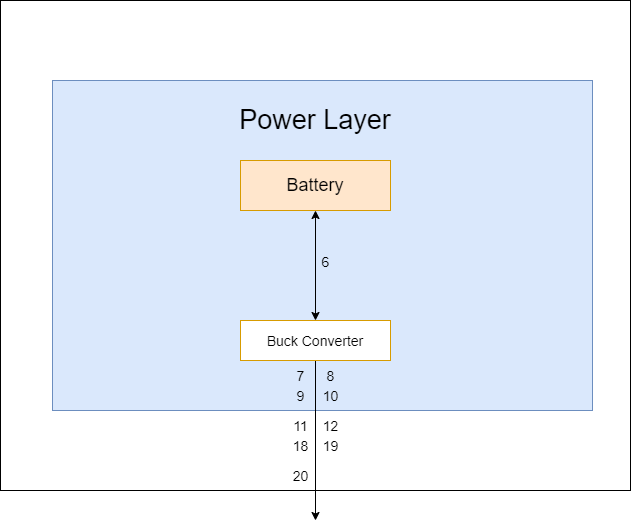
\includegraphics[width=0.60\textwidth]{images/Bat.png} % Image
 \caption{Battery Subsystem in Power Layer} % Caption
\end{figure}

\subsubsection{Subsystem Hardware}
The battery outputs around 36 volts rated at 8000mAh.

\subsubsection{Subsystem Operating System}
No operating system is used in this subsystem.

\subsubsection{Subsystem Software Dependencies}
No software is used in this subsystem

\subsubsection{Subsystem Programming Languages}
No programming languages are used in this subsystem.

\subsubsection{Subsystem Data Structures}
No data structures are used in this subsystem.

\subsubsection{Subsystem Data Processing}
No algorithms are used in this subsystem.

\subsection{Subsystem 2}
The entire module consists of a Li-Po battery to provide power to a Buck Converter which then powers the rest of the system. 

%%%%%%%%%%%%%%%%%%%%%%%%%%%%%%%%%%%%%%%%%%%%%%%%%%%%%%%%%%
%  BE SURE TO UPDATE THE IMAGE CAPTION
\begin{figure}[h!]
	\centering
 	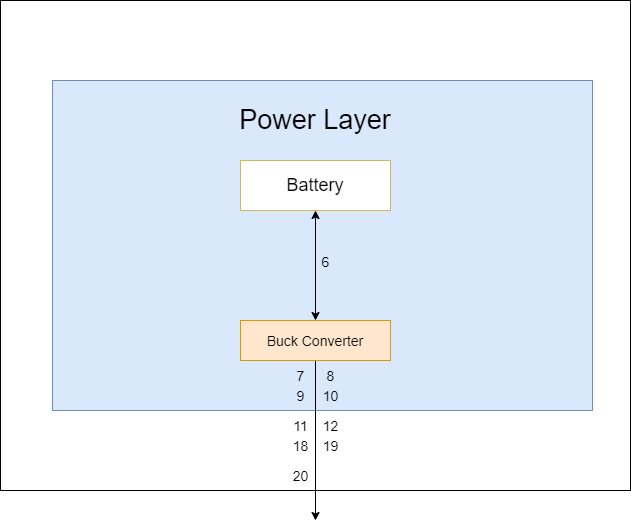
\includegraphics[width=0.60\textwidth]{images/Buck.png} % Image
 \caption{Buck Converter Subsystem in Power Layer} % Caption
\end{figure}

\subsubsection{Subsystem Hardware}
With an input voltage of 36 volts from the battery, the buck converters are able to output between 1.25V \textasciitilde 34V continuously.

\subsubsection{Subsystem Operating System}
No operating system is used in this subsystem.

\subsubsection{Subsystem Software Dependencies}
No software is used in this subsystem

\subsubsection{Subsystem Programming Languages}
No programming languages are used in this subsystem.

\subsubsection{Subsystem Data Structures}
No data structures are used in this subsystem.

\subsubsection{Subsystem Data Processing}
No algorithms are used in this subsystem.

\newpage
\section{Controls Software Layer Subsystems}
In this section, the layer is described in terms of the hardware and software design. Specific implementation details, such as hardware components, programming languages, software dependencies, operating systems, etc. should be discussed. Any unnecessary items can be omitted (for example, a pure software module without any specific hardware should not include a hardware subsection). The organization, titles, and content of the sections below can be modified as necessary for the project.

\subsection{Layer Hardware}
A description of any involved hardware components for the layer. For example, if each subsystem is a software process running on an embedded computer, discuss the specifics of that device here. Do not list a hardware component that only exists at the subsystem level (include it in the following sections).

\subsection{Layer Operating System}
A description of any operating systems required by the layer.

\subsection{Layer Software Dependencies}
A description of any software dependencies (libraries, frameworks, etc) required by the layer.

\subsection{Subsystem 1}
Describe at a high level the purpose and basic design of this subsystem. Is it a piece of hardware, a class, a web service, or something else? Note that each of the subsystem items below are meant to be specific to that subsystem and not a repeat of anything discussed above for the overall layer.

%%%%%%%%%%%%%%%%%%%%%%%%%%%%%%%%%%%%%%%%%%%%%%%%%%%%%%%%%%
%  BE SURE TO UPDATE THE IMAGE CAPTION
\begin{figure}[h!]
	\centering
 	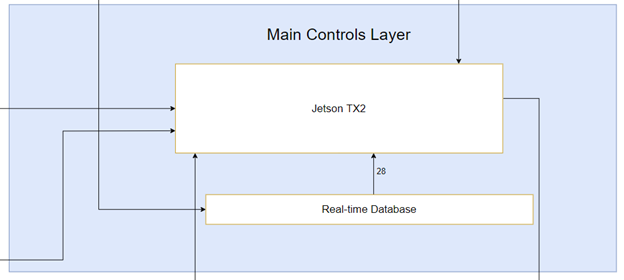
\includegraphics[width=0.60\textwidth]{images/MC.png} % Image
 \caption{Example subsystem description diagram} % Caption
\end{figure}

\subsubsection{Subsystem Hardware}
A description of any involved hardware components for the subsystem.

\subsubsection{Subsystem Operating System}
A description of any operating systems required by the subsystem.

\subsubsection{Subsystem Software Dependencies}
A description of any software dependencies (libraries, frameworks, design software for mechanical parts or circuits, etc) required by the subsystem.

\subsubsection{Subsystem Programming Languages}
A description of any programming languages used by the subsystem.

\subsubsection{Subsystem Data Structures}
A description of any classes or other data structures that are worth discussing for the subsystem. For example, data being transmitted from a microcontroller to a PC via USB should be first be assembled into packets. What is the structure of the packets?

\subsubsection{Subsystem Data Processing}
A description of any algorithms or processing strategies that are worth discussing for the subsystem. If you are implementing a well-known algorithm, list it. If it is something unique to this project, discuss it in greater detail.



\newpage
\section{Remote Control Layer Subsystems}
The sole purpose of this layer is to control the Turing Board. This layer is directly accessible to the user. This remote is in the form of an Android app or IOS app. This layer communicates with the Main Control layer adequately to propagate user commands. This layer also includes various features such as user authentication and user ride data analysis.

\subsection{Layer Hardware}
The remote controller for the Turing board is an app, which can be acquired from either the Android or IOS app store. This app runs on a smart phone capable of downloading apps.


\subsection{Layer Operating System}
The remote app can run on Android or IOS.

\subsection{Layer Software Dependencies}
The UI is connected to a Firebase back-end, which includes a real-time NoSQL database.

\subsection{Front-end UI and Main Control Communication}
The front-end UI is what the user sees on the Turing Board's app. The app is used as a remote controller for the Turing board. This is where different riding modes are selected. It is also where authentication and data analysis happens. The app communicates with our Firebase back-end which, in turn, communicates with the control layer (our embedded computer). The control layer then propagates the commands to the appropriate hardware.

%%%%%%%%%%%%%%%%%%%%%%%%%%%%%%%%%%%%%%%%%%%%%%%%%%%%%%%%%%
%  BE SURE TO UPDATE THE IMAGE CAPTION
\begin{figure}[h!]
	\centering
 	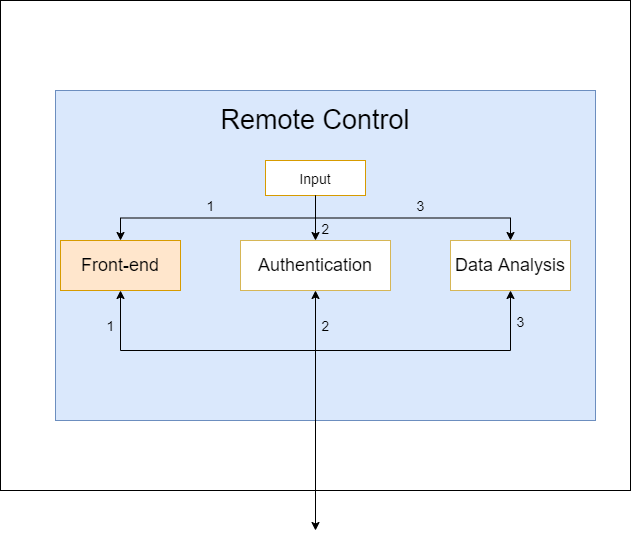
\includegraphics[width=0.60\textwidth]{images/UIJetsonCom.png} % Image
 \caption{Front-end UI and Main Control Communication Diagram} % Caption
\end{figure}

\subsubsection{Subsystem Hardware}
This system is accessed through the remote controller app, which requires a smartphone to run on.

\subsubsection{Subsystem Operating System}
Android or IOS is required to run the controller app.

\subsubsection{Subsystem Software Dependencies}
The front-end UI and Main Control communication subsystem depends on Wifi and a firebase back-end.

\subsubsection{Subsystem Programming Languages}
React-native and JavaScript.

\subsubsection{Subsystem Data Structures}
The data from the front-end UI and Main Control communication subsystem is received and sent to the back-end as JSON objects

\subsubsection{Subsystem Data Processing}
N/A

\subsection{Ride Data Analysis}
This subsystem of the remote controller layer will be information provided to the user after a ride. This information may include average speed of the ride, the duration of the ride, and the distance traveled. This information will be displayed on the app.

%%%%%%%%%%%%%%%%%%%%%%%%%%%%%%%%%%%%%%%%%%%%%%%%%%%%%%%%%%
%  BE SURE TO UPDATE THE IMAGE CAPTION
\begin{figure}[h!]
	\centering
 	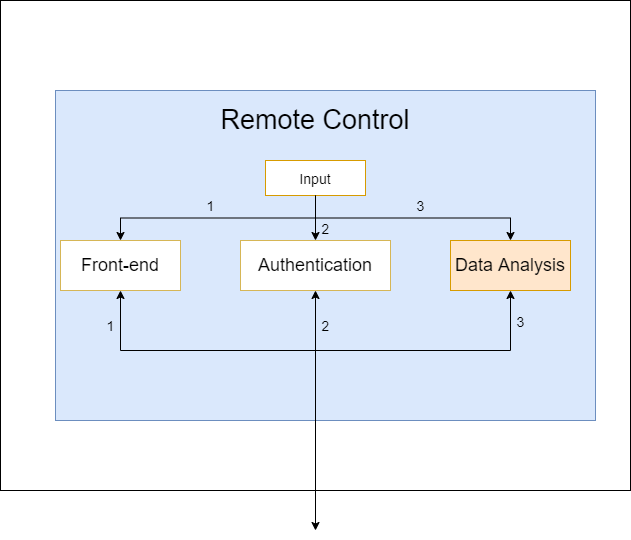
\includegraphics[width=0.60\textwidth]{images/dataAnalysis.png} % Image
 \caption{Ride Data Analysis Subsystem Diagram} % Caption
\end{figure}

\subsubsection{Subsystem Hardware}
N/A

\subsubsection{Subsystem Operating System}
This feature is within the controller app, so it runs on Android and IOS.

\subsubsection{Subsystem Software Dependencies}
The Ride Data Analysis subsystem depends on the controller app, and on a firebase NoSQL database.

\subsubsection{Subsystem Programming Languages}
React and JavaScript.

\subsubsection{Subsystem Data Structures}
The data from the Ride Data Analysis subsystem is received from the back-end as JSON objects.

\subsubsection{Subsystem Data Processing}
N/A

\subsection{Authentication}
When the user attempt to log into the app or sign up, the UI parses the login/signup information (name, email, password, etc.). The parsed data is then sent to a Firebase authentication API. The API, in turn, forwards a token to the app confirming status of the attempt, either a successful or unsuccessful login/sign up. The app then uses the data to render the UI accordingly.

%%%%%%%%%%%%%%%%%%%%%%%%%%%%%%%%%%%%%%%%%%%%%%%%%%%%%%%%%%
%  BE SURE TO UPDATE THE IMAGE CAPTION
\begin{figure}[h!]
	\centering
 	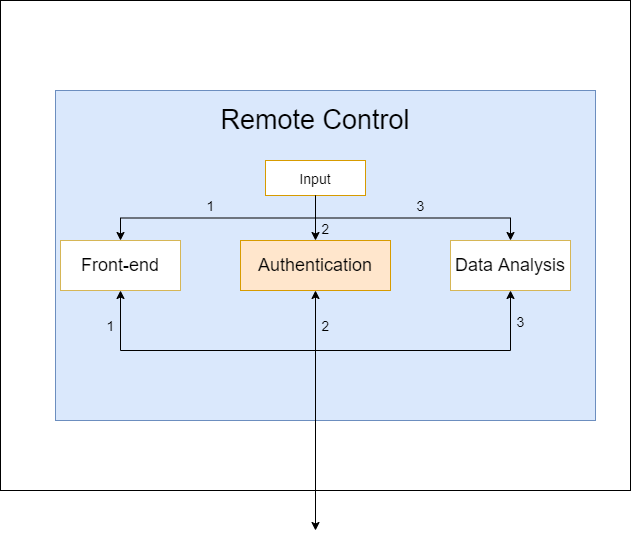
\includegraphics[width=0.60\textwidth]{images/Authentication.png} % Image
 \caption{Authentication subsystem diagram} % Caption
\end{figure}

\subsubsection{Subsystem Hardware}
N/A

\subsubsection{Subsystem Operating System}
N/A

\subsubsection{Subsystem Software Dependencies}
The Authentication subsystem depends on the app, and on the Firebase authentication API.

\subsubsection{Subsystem Programming Languages}
The front-end is written using React-native and JavaScript.

\subsubsection{Subsystem Data Structures}
The data from the Authentication subsystem is being sent to the back end as JSON objects.

\subsubsection{Subsystem Data Processing}
N/A

\newpage
\section{HMI Layer Subsystems}
This layer involves the various sensors and indicators that interact between the Turing Board and the user directly. This includes a load cell or force-sensing resistor for a weight sensor, a piezoelectric speaker, a printed ArUco symbol, a PWM-capable LED strip, a Tiva C Series Microcontroller, and various electrical components. The weight sensor, speaker, and LEDs communicate directly with the Tiva C Series, while the ArUco symbol is recognized by an Intel RealSense camera which sends the data to the Jetson TX2 via the CV Layer. The Tiva C Series is programmed using C and Assembly via Code Composer Studio 10, while the libraries used for the CV layer mainly use C++ and a generic IDE. This is capable of running on both Windows, MacOS, and Linux.

\subsection{Layer Hardware}
This layer uses a generic piezoelectric speaker (buzzer), a load cell or force-sensing resistor (weight sensor), a printed ArUco symbol generated online (follow anklet), a strip of PWM-capable LEDs approximately 10ft in length, a Tiva C Series, and various electrical components (MOSFETs, resistors, ADC, etc.).

\subsection{Layer Operating System}
N/A.

\subsection{Layer Software Dependencies}
This layer depends on code done in Code Composer Studio (v10.2) to program the Tiva C Series and drive the various HMI subsystems. We also used the site https://chev.me/arucogen/ to generate our ArUco symbol.

\subsection{Weight Sensor}
The weight sensor will be implemented as a safety feature primarily, with future uses in load carrying. When a user is riding on the board, it will detect if they fall off to initiate an emergency stop. When a user attempts to get on the board while in autonomous mode it will trigger an alert noise to notify the user it is not safe to ride.

\begin{figure}[h!]
	\centering
 	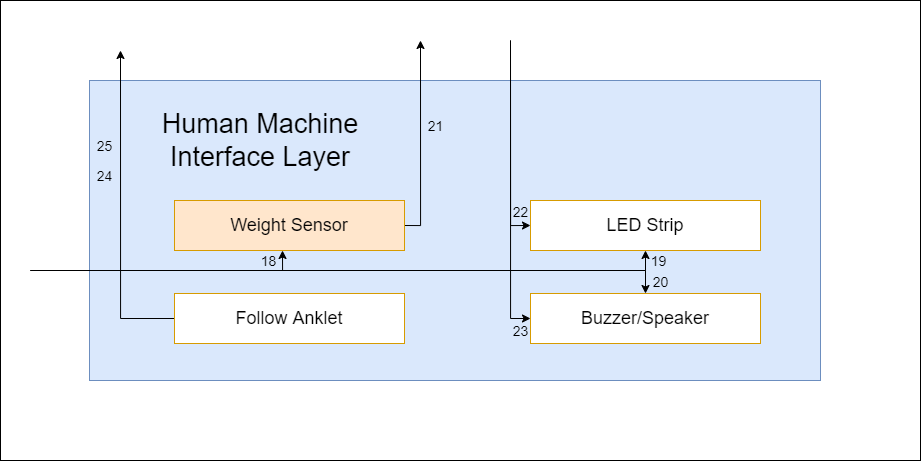
\includegraphics[width=0.60\textwidth]{images/Kendall/Weight Sensor.png}
 \caption{Weight Sensor Subsystem in HMI Layer}
\end{figure}

\subsubsection{Subsystem Hardware}
The weight sensor will implement either a generic load cell or force-sensing resistor in or order to determine the weight/pressure being generated by an item/person placed on top. This will detect and send any weight data to a Tiva C Series to parse and decode.

\subsubsection{Subsystem Operating System}
N/A.

\subsubsection{Subsystem Software Dependencies}
The weight sensor requires the Tiva C Series to read and parse any data. This, in turn, requires Code Composer Studio 10 to create code to parse/read the data and program the Tiva accordingly.

\subsubsection{Subsystem Programming Languages}
Code Composer Studio 10 has code written in C and Assembly.

\subsubsection{Subsystem Data Structures}
The data read in by the sensor is formed into 24-bit "packets" sent along a datastream to the Tiva running at 100kHz. This is done by transmitting one bit per clock using an ADC. This data, which correspond with an external linear force, is then read and parsed by the Tiva and any relevant data is passed to the other subsystems (LEDs and Buzzer/Speaker) to alert of a weight change.

\subsubsection{Subsystem Data Processing}
N/A.

\subsection{Buzzer/Speaker}
The buzzer/speaker will be used to alert the user if they attempt to step on the board when it is in an autonomous mode. When the weight sensor detects a person attempting to stand on the board when in autonomous mode, the buzzer will begin to sound an alert to notify the user it is unsafe to stand on it.

\begin{figure}[h!]
	\centering
 	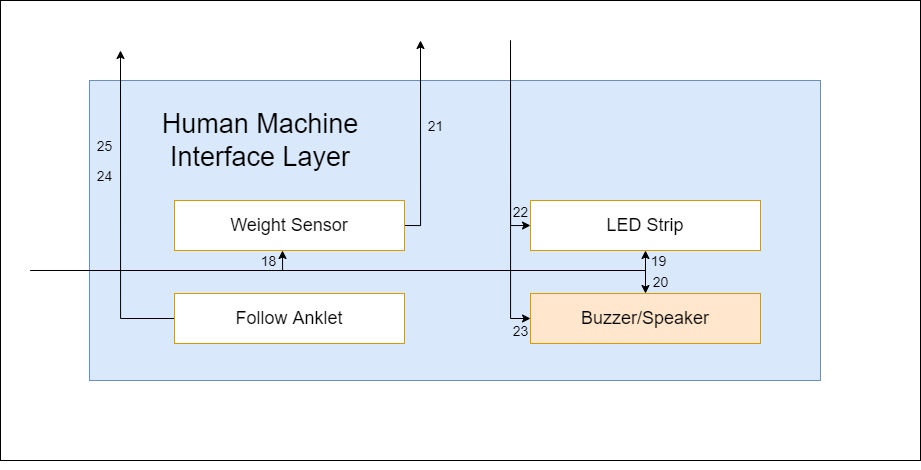
\includegraphics[width=0.60\textwidth]{images/Kendall/Buzzer.png}
 \caption{Buzzer/Speaker Subsystem in HMI Layer}
\end{figure}

\subsubsection{Subsystem Hardware}
This subsystem uses a generic piezoelectric speaker powered and run by a Tiva C Series to emit a sound as an alert on various conditions.

\subsubsection{Subsystem Operating System}
N/A.

\subsubsection{Subsystem Software Dependencies}
Code Composer Studio 10 is used to send signals to the piezoelectric speaker in order to emit a sound of a pre-determined frequency and length.

\subsubsection{Subsystem Programming Languages}
Code Composer Studio 10 has code written in C and Assembly.

\subsubsection{Subsystem Data Structures}
A signal is sent from the Tiva to the speaker using a 32-bit value to determine the frequency at which to emit the sound. The Tiva also uses a 32-bit variable to determine how long to emit the signal for before sending a stop command.

\subsubsection{Subsystem Data Processing}
N/A.

\subsection{LED Strip}
The LED strip will be used to indicate to the user what mode the Turing Board is currently in. These modes will be differentiated by implementing a different color for each mode. 

\begin{figure}[h!]
	\centering
 	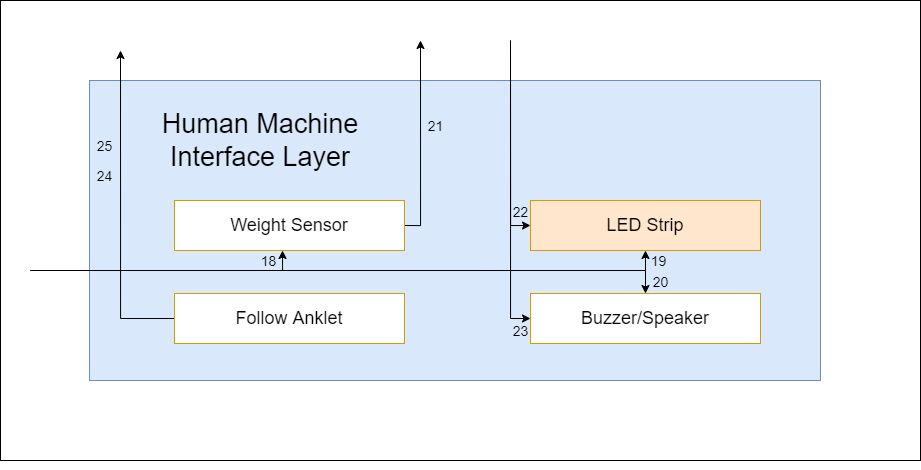
\includegraphics[width=0.60\textwidth]{images/Kendall/LED Strip.png}
 \caption{LED Strip Subsystem in HMI Layer}
\end{figure}

\subsubsection{Subsystem Hardware}
These LEDs are specifically PWM-capable and rated at up to 12V. It also implements a Tiva C Series to control the LEDs.

\subsubsection{Subsystem Operating System}
N/A.

\subsubsection{Subsystem Software Dependencies}
The LEDs are powered and controlled by the Tiva using Code Composer Studio.

\subsubsection{Subsystem Programming Languages}
Code Composer Studio 10 has code written in C and Assembly.

\subsubsection{Subsystem Data Structures}
The LEDs are each fed a 256-bit value corresponding to the Red, Blue, and Green data lines from the Tiva. This, in turn, activates the respective LED color to create various combinations based on each R/G/B input values.

\subsubsection{Subsystem Data Processing}
N/A.

\subsection{Follow Anklet}
The Anklet will be a worn feature used for the CV to track and follow the rider in follow-along mode.

\begin{figure}[h!]
	\centering
 	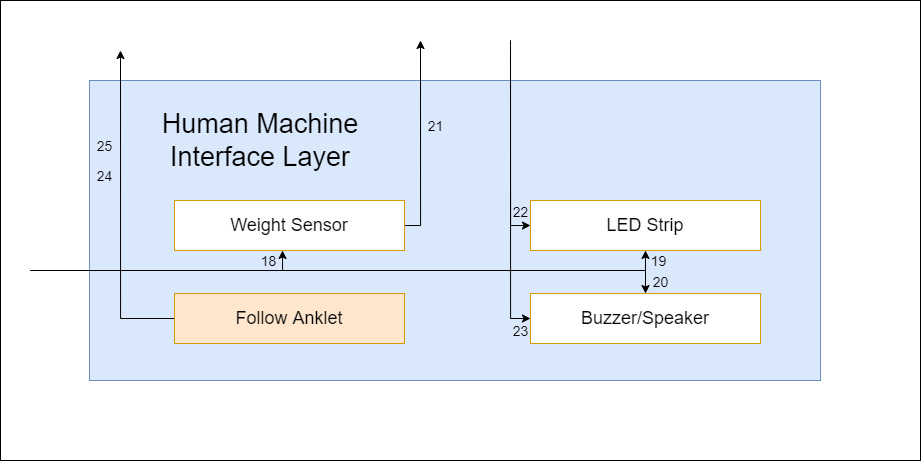
\includegraphics[width=0.60\textwidth]{images/Kendall/Anklet.png}
 \caption{Follow Anklet Subsystem in HMI Layer}
\end{figure}

\subsubsection{Subsystem Hardware}
This subsystem simply uses an ArUco symbol printed out on a strip of paper long enough to wrap around one's ankle.

\subsubsection{Subsystem Operating System}
N/A.

\subsubsection{Subsystem Software Dependencies}
This depends on the ArUco library based on the OpenCV library used to detect and track a generated symbol.

\subsubsection{Subsystem Programming Languages}
This uses C/C++ in the provided libraries required to detect and track the symbol.

\subsubsection{Subsystem Data Structures}
N/A.

\subsubsection{Subsystem Data Processing}
Uses an algorithm defined in the ArUco/OpenCV libraries to recognize and track the generated symbol.
\newpage
\section{Computer Vision Layer Subsystems}
This layer is the heart of the core autonomous functionalities of the Turing Board. We use computer
vision and depth imagery to determine the board’s surroundings and calculate the best path to move
forward. The user will have, strapped around their ankle, an anklet-like contraption consisting of a
pattern of ArUco markers for the Follow Along feature. This layer tracks the movement of the user
through the anklet to determine how to instruct the combination of motors to move so as to follow the
user at an appropriate pace. It is also responsible for detecting possible obstacles when operating on its
own to find the user as part of the Summon feature.
\subsection{Layer Hardware}
The required hardware components include the NVIDIA Jetson TX2 as the main compute module and the Intel RealSense  D432 Depth Camera.

\subsection{Layer Operating System}
The NVIDIA Jetson TX2 is running Ubuntu 18.04. 

\subsection{Layer Software Dependencies}
This layer requires the OpenCV v4.2.2 or higher compiled with cuDNN enabled. A more detailed and exhaustive list can be obtained from. https://github.com/TuringBoard/turing-board-vision/blob/main/Configuring%20the%20NVIDIA%20Jetson%20TX2.md.
% I know the text doesn't wrap to the next line for the link. Latex is stupid. I am not pressed about it. - Sahaj 

\subsection{RGB Imagery Subsystem
}
RGB Imagery of the front of the board is used as input in making various position specific calculations pertaining to navigation.

%%%%%%%%%%%%%%%%%%%%%%%%%%%%%%%%%%%%%%%%%%%%%%%%%%%%%%%%%%
%  BE SURE TO UPDATE THE IMAGE CAPTION
\begin{figure}[h!]
	\centering
 	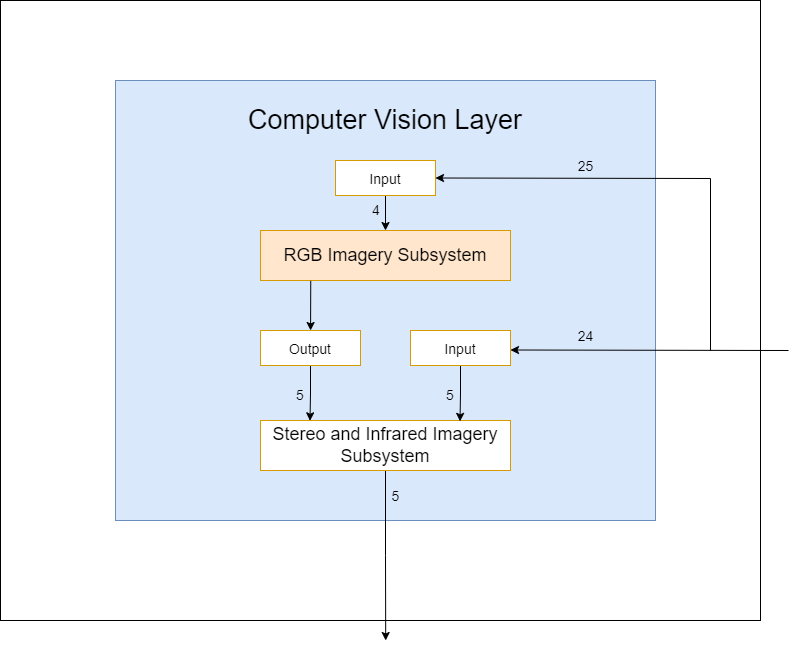
\includegraphics[width=0.60\textwidth]{DDS/images/CV_RGB.png} % Image
 \caption{CV Layer Subsystem} % Caption
\end{figure}

\subsubsection{Subsystem Hardware}
This subsystem requires the NVIDIA Jetson TX2 and the Intel RealSense  D432 Depth Camera.

\subsubsection{Subsystem Operating System}
Ubuntu 18.04.  

\subsubsection{Subsystem Software Dependencies}
This layer requires the OpenCV v4.2.2 or higher compiled with cuDNN enabled. A more detailed and exhaustive list can be obtained from. https://github.com/TuringBoard/turing-board-vision/blob/main/Configuring%20the%20NVIDIA%20Jetson%20TX2.md.
% I know the text doesn't wrap to the next line for the link. Latex is stupid. I am not pressed about it. - Sahaj 


\subsubsection{Subsystem Programming Languages}
Python 3.x.

\subsubsection{Subsystem Data Structures}
Arrays, HashMaps, Graphs, Trees.

\subsubsection{Subsystem Data Processing}
SIFT, RANSAC, Canny Edge Detection.







\subsection{Stereo Imagery Subsystem}
Stereo and Infrared Imagery of the front of the board is used as input in making various depth specific calculations pertaining to navigation.

%%%%%%%%%%%%%%%%%%%%%%%%%%%%%%%%%%%%%%%%%%%%%%%%%%%%%%%%%%
%  BE SURE TO UPDATE THE IMAGE CAPTION
\begin{figure}[h!]
	\centering
 	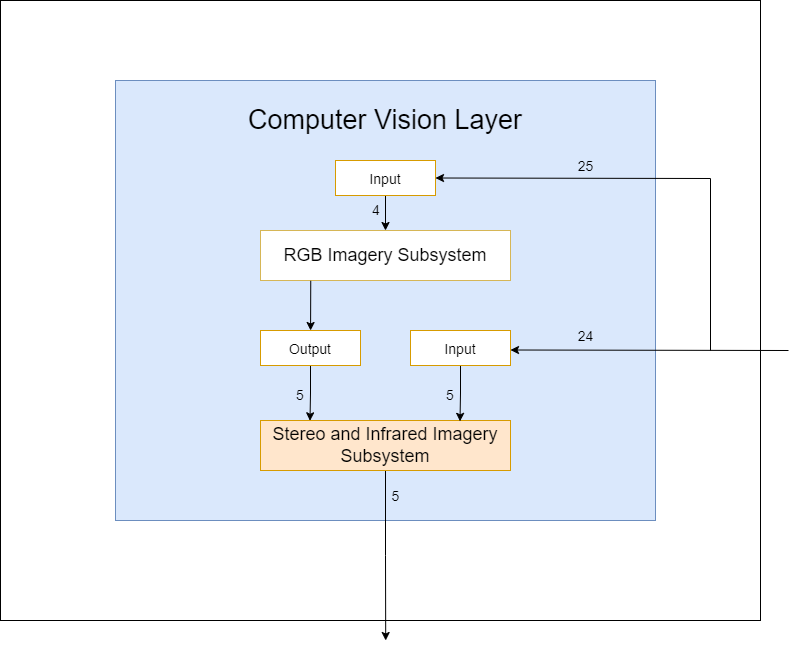
\includegraphics[width=0.60\textwidth]{DDS/images/CV_SIR.png} % Image
 \caption{CV Layer Subsystem} % Caption
\end{figure}

\subsubsection{Subsystem Hardware}
This subsystem requires the Intel RealSense  D432 Depth Camera.

\subsubsection{Subsystem Operating System}
N/A 

\subsubsection{Subsystem Software Dependencies}
pyrealsense: https://pypi.org/project/pyrealsense

librealsense: https://github.com/IntelRealSense/librealsense


\subsubsection{Subsystem Programming Languages}
Python 3.x.

\subsubsection{Subsystem Data Structures}
Arrays, HashMaps, Graphs, Trees.

\subsubsection{Subsystem Data Processing}
SIFT, RANSAC.



\newpage
\section{Appendix A}
Include any additional documents (CAD design, circuit schematics, etc) as an appendix as necessary.
\newpage

%%% References
\bibliographystyle{plain}
\bibliographystyle{reference/IEEEtran_custom}
\bibliography{reference/refs}{}

\end{document}